\documentclass[1p]{elsarticle_modified}
%\bibliographystyle{elsarticle-num}

%\usepackage[colorlinks]{hyperref}
%\usepackage{abbrmath_seonhwa} %\Abb, \Ascr, \Acal ,\Abf, \Afrak
\usepackage{amsfonts}
\usepackage{amssymb}
\usepackage{amsmath}
\usepackage{amsthm}
\usepackage{scalefnt}
\usepackage{amsbsy}
\usepackage{kotex}
\usepackage{caption}
\usepackage{subfig}
\usepackage{color}
\usepackage{graphicx}
\usepackage{xcolor} %% white, black, red, green, blue, cyan, magenta, yellow
\usepackage{float}
\usepackage{setspace}
\usepackage{hyperref}

\usepackage{tikz}
\usetikzlibrary{arrows}

\usepackage{multirow}
\usepackage{array} % fixed length table
\usepackage{hhline}

%%%%%%%%%%%%%%%%%%%%%
\makeatletter
\renewcommand*\env@matrix[1][\arraystretch]{%
	\edef\arraystretch{#1}%
	\hskip -\arraycolsep
	\let\@ifnextchar\new@ifnextchar
	\array{*\c@MaxMatrixCols c}}
\makeatother %https://tex.stackexchange.com/questions/14071/how-can-i-increase-the-line-spacing-in-a-matrix
%%%%%%%%%%%%%%%

\usepackage[normalem]{ulem}

\newcommand{\msout}[1]{\ifmmode\text{\sout{\ensuremath{#1}}}\else\sout{#1}\fi}
%SOURCE: \msout is \stkout macro in https://tex.stackexchange.com/questions/20609/strikeout-in-math-mode

\newcommand{\cancel}[1]{
	\ifmmode
	{\color{red}\msout{#1}}
	\else
	{\color{red}\sout{#1}}
	\fi
}

\newcommand{\add}[1]{
	{\color{blue}\uwave{#1}}
}

\newcommand{\replace}[2]{
	\ifmmode
	{\color{red}\msout{#1}}{\color{blue}\uwave{#2}}
	\else
	{\color{red}\sout{#1}}{\color{blue}\uwave{#2}}
	\fi
}

\newcommand{\Sol}{\mathcal{S}} %segment
\newcommand{\D}{D} %diagram
\newcommand{\A}{\mathcal{A}} %arc


%%%%%%%%%%%%%%%%%%%%%%%%%%%%%5 test

\def\sl{\operatorname{\textup{SL}}(2,\Cbb)}
\def\psl{\operatorname{\textup{PSL}}(2,\Cbb)}
\def\quan{\mkern 1mu \triangleright \mkern 1mu}

\theoremstyle{definition}
\newtheorem{thm}{Theorem}[section]
\newtheorem{prop}[thm]{Proposition}
\newtheorem{lem}[thm]{Lemma}
\newtheorem{ques}[thm]{Question}
\newtheorem{cor}[thm]{Corollary}
\newtheorem{defn}[thm]{Definition}
\newtheorem{exam}[thm]{Example}
\newtheorem{rmk}[thm]{Remark}
\newtheorem{alg}[thm]{Algorithm}

\newcommand{\I}{\sqrt{-1}}
\begin{document}

%\begin{frontmatter}
%
%\title{Boundary parabolic representations of knots up to 8 crossings}
%
%%% Group authors per affiliation:
%\author{Yunhi Cho} 
%\address{Department of Mathematics, University of Seoul, Seoul, Korea}
%\ead{yhcho@uos.ac.kr}
%
%
%\author{Seonhwa Kim} %\fnref{s_kim}}
%\address{Center for Geometry and Physics, Institute for Basic Science, Pohang, 37673, Korea}
%\ead{ryeona17@ibs.re.kr}
%
%\author{Hyuk Kim}
%\address{Department of Mathematical Sciences, Seoul National University, Seoul 08826, Korea}
%\ead{hyukkim@snu.ac.kr}
%
%\author{Seokbeom Yoon}
%\address{Department of Mathematical Sciences, Seoul National University, Seoul, 08826,  Korea}
%\ead{sbyoon15@snu.ac.kr}
%
%\begin{abstract}
%We find all boundary parabolic representation of knots up to 8 crossings.
%
%\end{abstract}
%\begin{keyword}
%    \MSC[2010] 57M25 
%\end{keyword}
%
%\end{frontmatter}

%\linenumbers
%\tableofcontents
%
\newcommand\colored[1]{\textcolor{white}{\rule[-0.35ex]{0.8em}{1.4ex}}\kern-0.8em\color{red} #1}%
%\newcommand\colored[1]{\textcolor{white}{ #1}\kern-2.17ex	\textcolor{white}{ #1}\kern-1.81ex	\textcolor{white}{ #1}\kern-2.15ex\color{red}#1	}

{\Large $\underline{12a_{0434}~(K12a_{0434})}$}

\setlength{\tabcolsep}{10pt}
\renewcommand{\arraystretch}{1.6}
\vspace{1cm}\begin{tabular}{m{100pt}>{\centering\arraybackslash}m{274pt}}
\multirow{5}{120pt}{
	\centering
	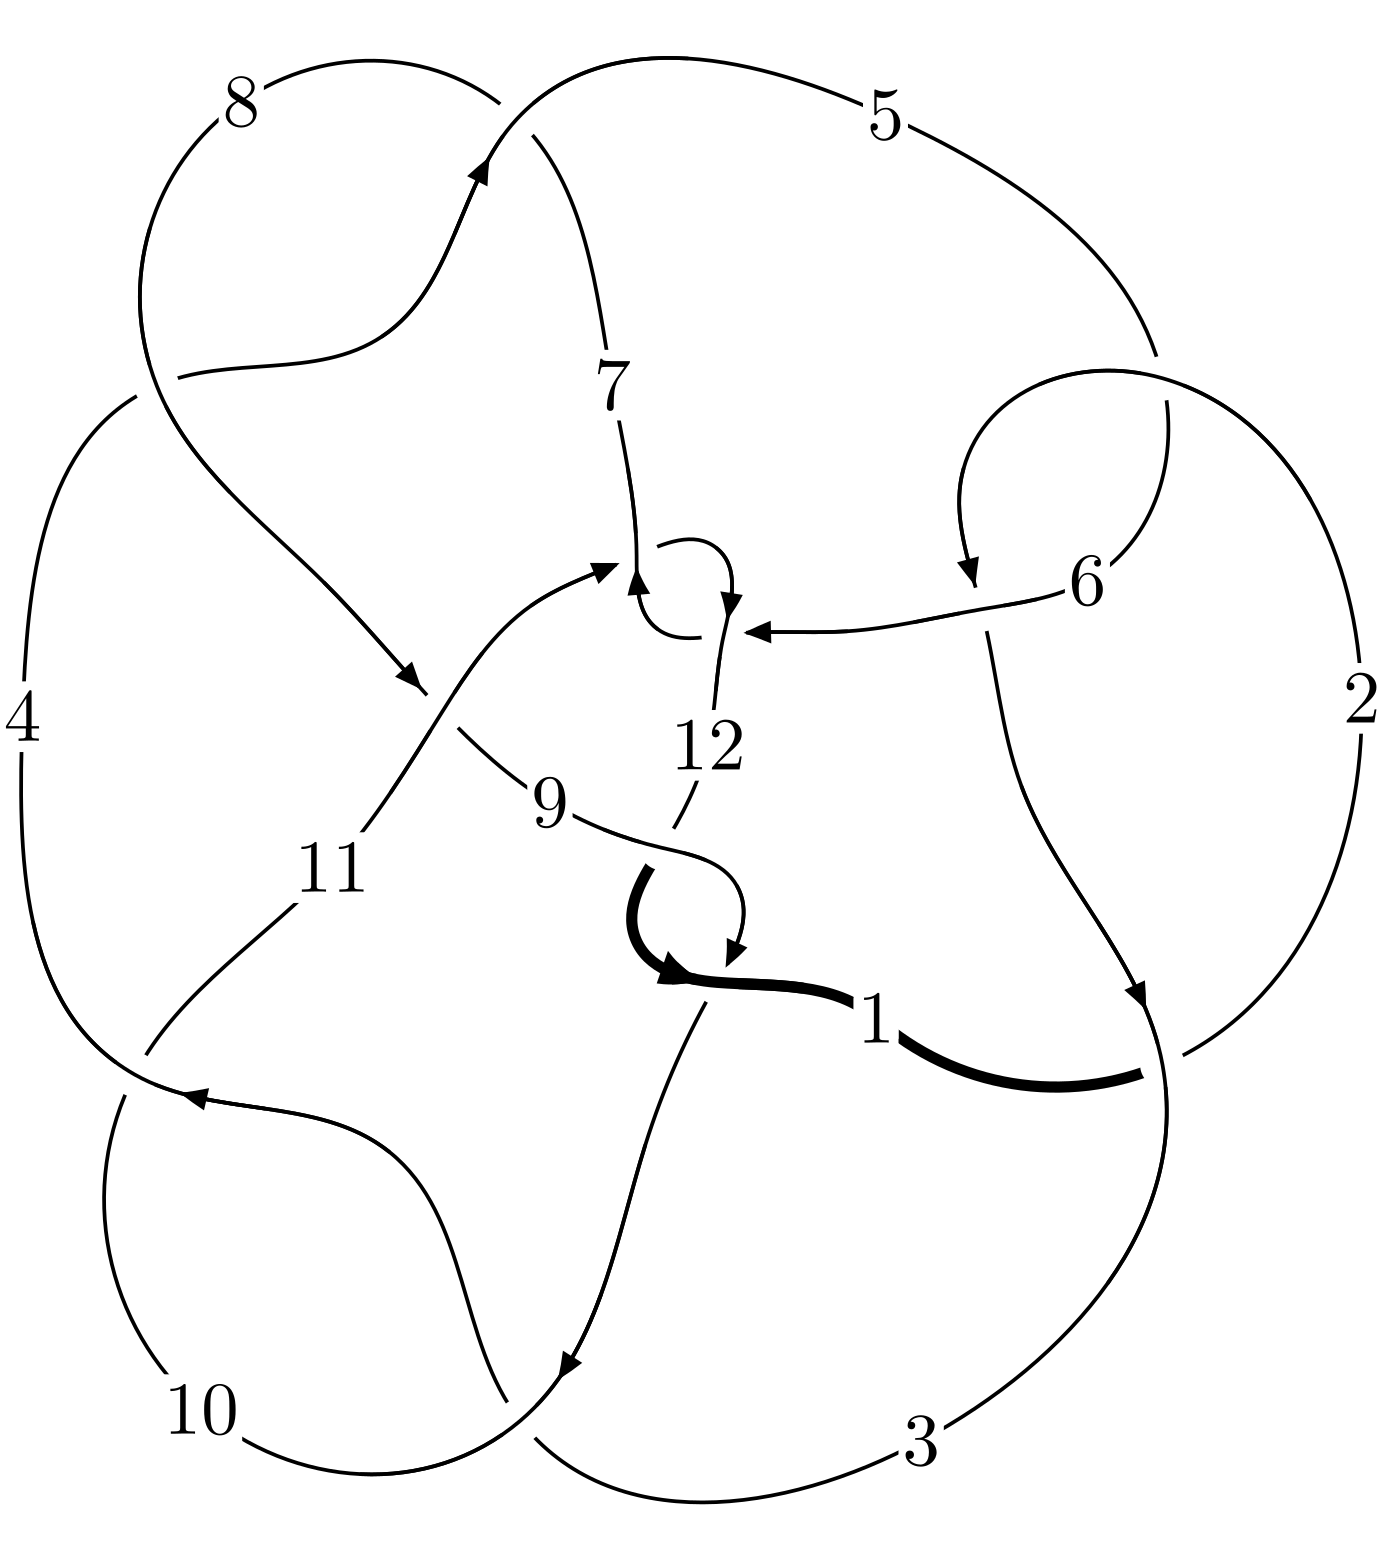
\includegraphics[width=112pt]{../../../GIT/diagram.site/Diagrams/png/1235_12a_0434.png}\\
\ \ \ A knot diagram\footnotemark}&
\allowdisplaybreaks
\textbf{Linearized knot diagam} \\
\cline{2-2}
 &
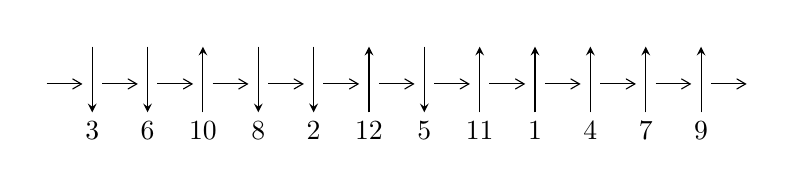
\begin{tikzpicture}[x=20pt, y=17pt]
	% nodes
	\node (C0) at (0, 0) {};
	\node (C1) at (1, 0) {};
	\node (C1U) at (1, +1) {};
	\node (C1D) at (1, -1) {3};

	\node (C2) at (2, 0) {};
	\node (C2U) at (2, +1) {};
	\node (C2D) at (2, -1) {6};

	\node (C3) at (3, 0) {};
	\node (C3U) at (3, +1) {};
	\node (C3D) at (3, -1) {10};

	\node (C4) at (4, 0) {};
	\node (C4U) at (4, +1) {};
	\node (C4D) at (4, -1) {8};

	\node (C5) at (5, 0) {};
	\node (C5U) at (5, +1) {};
	\node (C5D) at (5, -1) {2};

	\node (C6) at (6, 0) {};
	\node (C6U) at (6, +1) {};
	\node (C6D) at (6, -1) {12};

	\node (C7) at (7, 0) {};
	\node (C7U) at (7, +1) {};
	\node (C7D) at (7, -1) {5};

	\node (C8) at (8, 0) {};
	\node (C8U) at (8, +1) {};
	\node (C8D) at (8, -1) {11};

	\node (C9) at (9, 0) {};
	\node (C9U) at (9, +1) {};
	\node (C9D) at (9, -1) {1};

	\node (C10) at (10, 0) {};
	\node (C10U) at (10, +1) {};
	\node (C10D) at (10, -1) {4};

	\node (C11) at (11, 0) {};
	\node (C11U) at (11, +1) {};
	\node (C11D) at (11, -1) {7};

	\node (C12) at (12, 0) {};
	\node (C12U) at (12, +1) {};
	\node (C12D) at (12, -1) {9};
	\node (C13) at (13, 0) {};

	% arrows
	\draw[->,>={angle 60}]
	(C0) edge (C1) (C1) edge (C2) (C2) edge (C3) (C3) edge (C4) (C4) edge (C5) (C5) edge (C6) (C6) edge (C7) (C7) edge (C8) (C8) edge (C9) (C9) edge (C10) (C10) edge (C11) (C11) edge (C12) (C12) edge (C13) ;	\draw[->,>=stealth]
	(C1U) edge (C1D) (C2U) edge (C2D) (C3D) edge (C3U) (C4U) edge (C4D) (C5U) edge (C5D) (C6D) edge (C6U) (C7U) edge (C7D) (C8D) edge (C8U) (C9D) edge (C9U) (C10D) edge (C10U) (C11D) edge (C11U) (C12D) edge (C12U) ;
	\end{tikzpicture} \\
\hhline{~~} \\& 
\textbf{Solving Sequence} \\ \cline{2-2} 
 &
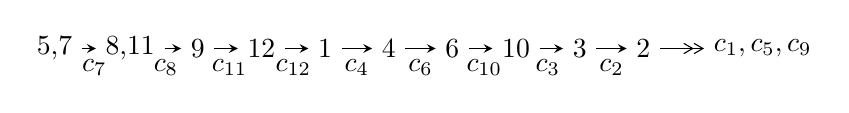
\begin{tikzpicture}[x=23pt, y=7pt]
	% node
	\node (A0) at (-1/8, 0) {5,7};
	\node (A1) at (17/16, 0) {8,11};
	\node (A2) at (17/8, 0) {9};
	\node (A3) at (25/8, 0) {12};
	\node (A4) at (33/8, 0) {1};
	\node (A5) at (41/8, 0) {4};
	\node (A6) at (49/8, 0) {6};
	\node (A7) at (57/8, 0) {10};
	\node (A8) at (65/8, 0) {3};
	\node (A9) at (73/8, 0) {2};
	\node (C1) at (1/2, -1) {$c_{7}$};
	\node (C2) at (13/8, -1) {$c_{8}$};
	\node (C3) at (21/8, -1) {$c_{11}$};
	\node (C4) at (29/8, -1) {$c_{12}$};
	\node (C5) at (37/8, -1) {$c_{4}$};
	\node (C6) at (45/8, -1) {$c_{6}$};
	\node (C7) at (53/8, -1) {$c_{10}$};
	\node (C8) at (61/8, -1) {$c_{3}$};
	\node (C9) at (69/8, -1) {$c_{2}$};
	\node (A10) at (11, 0) {$c_{1},c_{5},c_{9}$};

	% edge
	\draw[->,>=stealth]	
	(A0) edge (A1) (A1) edge (A2) (A2) edge (A3) (A3) edge (A4) (A4) edge (A5) (A5) edge (A6) (A6) edge (A7) (A7) edge (A8) (A8) edge (A9) ;
	\draw[->>,>={angle 60}]	
	(A9) edge (A10);
\end{tikzpicture} \\ 

\end{tabular} \\

\footnotetext{
The image of knot diagram is generated by the software ``\textbf{Draw programme}" developed by Andrew Bartholomew(\url{http://www.layer8.co.uk/maths/draw/index.htm\#Running-draw}), where we modified some parts for our purpose(\url{https://github.com/CATsTAILs/LinksPainter}).
}\phantom \\ \newline 
\centering \textbf{Ideals for irreducible components\footnotemark of $X_{\text{par}}$} 
 
\begin{align*}
I^u_{1}&=\langle 
9.71302\times10^{556} u^{125}-6.76323\times10^{557} u^{124}+\cdots+1.54432\times10^{557} b+9.08091\times10^{559},\\
\phantom{I^u_{1}}&\phantom{= \langle  }1.44998\times10^{560} u^{125}-9.16910\times10^{559} u^{124}+\cdots+3.22764\times10^{559} a-3.36668\times10^{562},\\
\phantom{I^u_{1}}&\phantom{= \langle  }u^{126}-2 u^{125}+\cdots-347 u-209\rangle \\
I^u_{2}&=\langle 
-2.54767\times10^{19} u^{28}-8.03536\times10^{19} u^{27}+\cdots+1.20106\times10^{19} b+1.25244\times10^{20},\\
\phantom{I^u_{2}}&\phantom{= \langle  }-4.39555\times10^{19} u^{28}-1.42315\times10^{20} u^{27}+\cdots+1.20106\times10^{19} a+2.23950\times10^{20},\;u^{29}+3 u^{28}+\cdots-8 u+1\rangle \\
\\
\end{align*}
\raggedright * 2 irreducible components of $\dim_{\mathbb{C}}=0$, with total 155 representations.\\
\footnotetext{All coefficients of polynomials are rational numbers. But the coefficients are sometimes approximated in decimal forms when there is not enough margin.}
\newpage
\renewcommand{\arraystretch}{1}
\centering \section*{I. $I^u_{1}= \langle 9.71\times10^{556} u^{125}-6.76\times10^{557} u^{124}+\cdots+1.54\times10^{557} b+9.08\times10^{559},\;1.45\times10^{560} u^{125}-9.17\times10^{559} u^{124}+\cdots+3.23\times10^{559} a-3.37\times10^{562},\;u^{126}-2 u^{125}+\cdots-347 u-209 \rangle$}
\flushleft \textbf{(i) Arc colorings}\\
\begin{tabular}{m{7pt} m{180pt} m{7pt} m{180pt} }
\flushright $a_{5}=$&$\begin{pmatrix}0\\u\end{pmatrix}$ \\
\flushright $a_{7}=$&$\begin{pmatrix}1\\0\end{pmatrix}$ \\
\flushright $a_{8}=$&$\begin{pmatrix}1\\u^2\end{pmatrix}$ \\
\flushright $a_{11}=$&$\begin{pmatrix}-4.49239 u^{125}+2.84081 u^{124}+\cdots+2658.84 u+1043.08\\-0.628950 u^{125}+4.37941 u^{124}+\cdots-902.391 u-588.019\end{pmatrix}$ \\
\flushright $a_{9}=$&$\begin{pmatrix}12.6795 u^{125}-29.5835 u^{124}+\cdots-675.654 u+926.547\\1.46707 u^{125}-5.94916 u^{124}+\cdots+701.891 u+556.492\end{pmatrix}$ \\
\flushright $a_{12}=$&$\begin{pmatrix}-5.12134 u^{125}+7.22022 u^{124}+\cdots+1756.45 u+455.061\\-0.628950 u^{125}+4.37941 u^{124}+\cdots-902.391 u-588.019\end{pmatrix}$ \\
\flushright $a_{1}=$&$\begin{pmatrix}13.0154 u^{125}-29.2173 u^{124}+\cdots-1067.78 u+742.305\\1.98155 u^{125}-7.75311 u^{124}+\cdots+858.066 u+702.323\end{pmatrix}$ \\
\flushright $a_{4}=$&$\begin{pmatrix}u\\u^3+u\end{pmatrix}$ \\
\flushright $a_{6}=$&$\begin{pmatrix}-0.520880 u^{125}+3.53209 u^{124}+\cdots-707.275 u-448.096\\2.95348 u^{125}-7.44049 u^{124}+\cdots-31.7519 u+284.495\end{pmatrix}$ \\
\flushright $a_{10}=$&$\begin{pmatrix}-5.52684 u^{125}+6.83560 u^{124}+\cdots+2194.45 u+666.015\\-0.327914 u^{125}+3.67582 u^{124}+\cdots-914.697 u-562.572\end{pmatrix}$ \\
\flushright $a_{3}=$&$\begin{pmatrix}2.41465 u^{125}-0.517100 u^{124}+\cdots-1699.20 u-736.916\\-0.803163 u^{125}-0.505149 u^{124}+\cdots+735.110 u+358.811\end{pmatrix}$ \\
\flushright $a_{2}=$&$\begin{pmatrix}0.624449 u^{125}-1.81920 u^{124}+\cdots+93.7798 u+108.872\\-3.25032 u^{125}+6.88477 u^{124}+\cdots+412.972 u-89.4386\end{pmatrix}$\\&\end{tabular}
\flushleft \textbf{(ii) Obstruction class $= -1$}\\~\\
\flushleft \textbf{(iii) Cusp Shapes $= -10.7598 u^{125}+12.4868 u^{124}+\cdots+4646.15 u+1557.69$}\\~\\
\newpage\renewcommand{\arraystretch}{1}
\flushleft \textbf{(iv) u-Polynomials at the component}\newline \\
\begin{tabular}{m{50pt}|m{274pt}}
Crossings & \hspace{64pt}u-Polynomials at each crossing \\
\hline $$\begin{aligned}c_{1}\end{aligned}$$&$\begin{aligned}
&u^{126}+46 u^{125}+\cdots+113201 u+1156
\end{aligned}$\\
\hline $$\begin{aligned}c_{2},c_{5}\end{aligned}$$&$\begin{aligned}
&u^{126}+4 u^{125}+\cdots+435 u-34
\end{aligned}$\\
\hline $$\begin{aligned}c_{3},c_{10}\end{aligned}$$&$\begin{aligned}
&u^{126}+u^{125}+\cdots-43434 u+3284
\end{aligned}$\\
\hline $$\begin{aligned}c_{4},c_{7}\end{aligned}$$&$\begin{aligned}
&u^{126}-2 u^{125}+\cdots-347 u-209
\end{aligned}$\\
\hline $$\begin{aligned}c_{6},c_{11}\end{aligned}$$&$\begin{aligned}
&u^{126}-10 u^{125}+\cdots-2573 u-589
\end{aligned}$\\
\hline $$\begin{aligned}c_{8}\end{aligned}$$&$\begin{aligned}
&u^{126}+16 u^{125}+\cdots-8670271 u-644753
\end{aligned}$\\
\hline $$\begin{aligned}c_{9},c_{12}\end{aligned}$$&$\begin{aligned}
&u^{126}-44 u^{124}+\cdots+448775 u-34921
\end{aligned}$\\
\hline
\end{tabular}\\~\\
\newpage\renewcommand{\arraystretch}{1}
\flushleft \textbf{(v) Riley Polynomials at the component}\newline \\
\begin{tabular}{m{50pt}|m{274pt}}
Crossings & \hspace{64pt}Riley Polynomials at each crossing \\
\hline $$\begin{aligned}c_{1}\end{aligned}$$&$\begin{aligned}
&y^{126}+82 y^{125}+\cdots-2963728001 y+1336336
\end{aligned}$\\
\hline $$\begin{aligned}c_{2},c_{5}\end{aligned}$$&$\begin{aligned}
&y^{126}-46 y^{125}+\cdots-113201 y+1156
\end{aligned}$\\
\hline $$\begin{aligned}c_{3},c_{10}\end{aligned}$$&$\begin{aligned}
&y^{126}-85 y^{125}+\cdots-747181100 y+10784656
\end{aligned}$\\
\hline $$\begin{aligned}c_{4},c_{7}\end{aligned}$$&$\begin{aligned}
&y^{126}+80 y^{125}+\cdots-2175715 y+43681
\end{aligned}$\\
\hline $$\begin{aligned}c_{6},c_{11}\end{aligned}$$&$\begin{aligned}
&y^{126}+40 y^{125}+\cdots+4386903 y+346921
\end{aligned}$\\
\hline $$\begin{aligned}c_{8}\end{aligned}$$&$\begin{aligned}
&y^{126}-44 y^{125}+\cdots-35320777977971 y+415706431009
\end{aligned}$\\
\hline $$\begin{aligned}c_{9},c_{12}\end{aligned}$$&$\begin{aligned}
&y^{126}-88 y^{125}+\cdots+7738747697 y+1219476241
\end{aligned}$\\
\hline
\end{tabular}\\~\\
\newpage\flushleft \textbf{(vi) Complex Volumes and Cusp Shapes}
$$\begin{array}{c|c|c}  
\text{Solutions to }I^u_{1}& \I (\text{vol} + \sqrt{-1}CS) & \text{Cusp shape}\\
 \hline 
\begin{aligned}
u &= -0.918554 + 0.382892 I \\
a &= \phantom{-}0.069082 - 0.707553 I \\
b &= \phantom{-}0.716442 - 0.348828 I\end{aligned}
 & \phantom{-}6.33888 + 7.34118 I & \phantom{-0.000000 } 0 \\ \hline\begin{aligned}
u &= -0.918554 - 0.382892 I \\
a &= \phantom{-}0.069082 + 0.707553 I \\
b &= \phantom{-}0.716442 + 0.348828 I\end{aligned}
 & \phantom{-}6.33888 - 7.34118 I & \phantom{-0.000000 } 0 \\ \hline\begin{aligned}
u &= -0.024941 + 0.966430 I \\
a &= \phantom{-}4.44092 + 0.33646 I \\
b &= -3.96951 - 0.52328 I\end{aligned}
 & \phantom{-}3.51148 - 2.18628 I & \phantom{-0.000000 } 0 \\ \hline\begin{aligned}
u &= -0.024941 - 0.966430 I \\
a &= \phantom{-}4.44092 - 0.33646 I \\
b &= -3.96951 + 0.52328 I\end{aligned}
 & \phantom{-}3.51148 + 2.18628 I & \phantom{-0.000000 } 0 \\ \hline\begin{aligned}
u &= \phantom{-}0.945274 + 0.458726 I \\
a &= \phantom{-}0.326155 + 0.330779 I \\
b &= \phantom{-}0.333947 + 1.100140 I\end{aligned}
 & -4.21417 + 2.72263 I & \phantom{-0.000000 } 0 \\ \hline\begin{aligned}
u &= \phantom{-}0.945274 - 0.458726 I \\
a &= \phantom{-}0.326155 - 0.330779 I \\
b &= \phantom{-}0.333947 - 1.100140 I\end{aligned}
 & -4.21417 - 2.72263 I & \phantom{-0.000000 } 0 \\ \hline\begin{aligned}
u &= \phantom{-}0.057623 + 1.060710 I \\
a &= -1.177790 + 0.181081 I \\
b &= \phantom{-}0.40022 - 1.49417 I\end{aligned}
 & \phantom{-}1.74556 - 3.88859 I & \phantom{-0.000000 } 0 \\ \hline\begin{aligned}
u &= \phantom{-}0.057623 - 1.060710 I \\
a &= -1.177790 - 0.181081 I \\
b &= \phantom{-}0.40022 + 1.49417 I\end{aligned}
 & \phantom{-}1.74556 + 3.88859 I & \phantom{-0.000000 } 0 \\ \hline\begin{aligned}
u &= \phantom{-}0.078826 + 1.067810 I \\
a &= \phantom{-}2.62867 + 0.05998 I \\
b &= -0.336959 - 0.797761 I\end{aligned}
 & \phantom{-}9.49842 - 0.50398 I & \phantom{-0.000000 } 0 \\ \hline\begin{aligned}
u &= \phantom{-}0.078826 - 1.067810 I \\
a &= \phantom{-}2.62867 - 0.05998 I \\
b &= -0.336959 + 0.797761 I\end{aligned}
 & \phantom{-}9.49842 + 0.50398 I & \phantom{-0.000000 } 0\\
 \hline 
 \end{array}$$\newpage$$\begin{array}{c|c|c}  
\text{Solutions to }I^u_{1}& \I (\text{vol} + \sqrt{-1}CS) & \text{Cusp shape}\\
 \hline 
\begin{aligned}
u &= \phantom{-}0.040872 + 1.074960 I \\
a &= \phantom{-}1.83280 + 1.40801 I \\
b &= -0.315733 + 1.092720 I\end{aligned}
 & \phantom{-}6.20931 - 7.12639 I & \phantom{-0.000000 } 0 \\ \hline\begin{aligned}
u &= \phantom{-}0.040872 - 1.074960 I \\
a &= \phantom{-}1.83280 - 1.40801 I \\
b &= -0.315733 - 1.092720 I\end{aligned}
 & \phantom{-}6.20931 + 7.12639 I & \phantom{-0.000000 } 0 \\ \hline\begin{aligned}
u &= \phantom{-}0.879333 + 0.277785 I \\
a &= -0.1077040 - 0.0740349 I \\
b &= -0.570900 - 1.171590 I\end{aligned}
 & -0.74106 + 7.37313 I & \phantom{-0.000000 } 0 \\ \hline\begin{aligned}
u &= \phantom{-}0.879333 - 0.277785 I \\
a &= -0.1077040 + 0.0740349 I \\
b &= -0.570900 + 1.171590 I\end{aligned}
 & -0.74106 - 7.37313 I & \phantom{-0.000000 } 0 \\ \hline\begin{aligned}
u &= \phantom{-}0.024557 + 1.078400 I \\
a &= -1.28679 - 0.60675 I \\
b &= \phantom{-}0.86022 + 1.45214 I\end{aligned}
 & \phantom{-}3.25361 - 0.82524 I & \phantom{-0.000000 } 0 \\ \hline\begin{aligned}
u &= \phantom{-}0.024557 - 1.078400 I \\
a &= -1.28679 + 0.60675 I \\
b &= \phantom{-}0.86022 - 1.45214 I\end{aligned}
 & \phantom{-}3.25361 + 0.82524 I & \phantom{-0.000000 } 0 \\ \hline\begin{aligned}
u &= -0.907784 + 0.114565 I \\
a &= -0.0391522 + 0.0596593 I \\
b &= -0.502144 + 1.027850 I\end{aligned}
 & \phantom{-}0.01352 - 2.04886 I & \phantom{-0.000000 } 0 \\ \hline\begin{aligned}
u &= -0.907784 - 0.114565 I \\
a &= -0.0391522 - 0.0596593 I \\
b &= -0.502144 - 1.027850 I\end{aligned}
 & \phantom{-}0.01352 + 2.04886 I & \phantom{-0.000000 } 0 \\ \hline\begin{aligned}
u &= \phantom{-}0.427894 + 0.998851 I \\
a &= \phantom{-}1.53351 - 0.34685 I \\
b &= -0.217091 + 1.043910 I\end{aligned}
 & -3.69560 - 0.52746 I & \phantom{-0.000000 } 0 \\ \hline\begin{aligned}
u &= \phantom{-}0.427894 - 0.998851 I \\
a &= \phantom{-}1.53351 + 0.34685 I \\
b &= -0.217091 - 1.043910 I\end{aligned}
 & -3.69560 + 0.52746 I & \phantom{-0.000000 } 0\\
 \hline 
 \end{array}$$\newpage$$\begin{array}{c|c|c}  
\text{Solutions to }I^u_{1}& \I (\text{vol} + \sqrt{-1}CS) & \text{Cusp shape}\\
 \hline 
\begin{aligned}
u &= -0.865598 + 0.276073 I \\
a &= \phantom{-}0.254193 - 0.232814 I \\
b &= \phantom{-}0.032276 - 0.962160 I\end{aligned}
 & -2.07762 + 1.21796 I & \phantom{-0.000000 } 0 \\ \hline\begin{aligned}
u &= -0.865598 - 0.276073 I \\
a &= \phantom{-}0.254193 + 0.232814 I \\
b &= \phantom{-}0.032276 + 0.962160 I\end{aligned}
 & -2.07762 - 1.21796 I & \phantom{-0.000000 } 0 \\ \hline\begin{aligned}
u &= \phantom{-}0.018444 + 1.092110 I \\
a &= -1.44523 - 0.26685 I \\
b &= \phantom{-}0.750592 + 0.862940 I\end{aligned}
 & \phantom{-}3.38500 - 0.51199 I & \phantom{-0.000000 } 0 \\ \hline\begin{aligned}
u &= \phantom{-}0.018444 - 1.092110 I \\
a &= -1.44523 + 0.26685 I \\
b &= \phantom{-}0.750592 - 0.862940 I\end{aligned}
 & \phantom{-}3.38500 + 0.51199 I & \phantom{-0.000000 } 0 \\ \hline\begin{aligned}
u &= -0.897663\phantom{ +0.000000I} \\
a &= -0.223552\phantom{ +0.000000I} \\
b &= \phantom{-}0.882497\phantom{ +0.000000I}\end{aligned}
 & \phantom{-}1.97369\phantom{ +0.000000I} & \phantom{-0.000000 } 0 \\ \hline\begin{aligned}
u &= \phantom{-}0.436929 + 1.023820 I \\
a &= -1.18070 - 1.02393 I \\
b &= \phantom{-}0.380839 - 1.050540 I\end{aligned}
 & \phantom{-}3.26110 - 5.44389 I & \phantom{-0.000000 } 0 \\ \hline\begin{aligned}
u &= \phantom{-}0.436929 - 1.023820 I \\
a &= -1.18070 + 1.02393 I \\
b &= \phantom{-}0.380839 + 1.050540 I\end{aligned}
 & \phantom{-}3.26110 + 5.44389 I & \phantom{-0.000000 } 0 \\ \hline\begin{aligned}
u &= \phantom{-}0.030154 + 1.130170 I \\
a &= \phantom{-}1.41025 + 1.05759 I \\
b &= -1.45272 - 1.42233 I\end{aligned}
 & \phantom{-}2.69190 + 2.06472 I & \phantom{-0.000000 } 0 \\ \hline\begin{aligned}
u &= \phantom{-}0.030154 - 1.130170 I \\
a &= \phantom{-}1.41025 - 1.05759 I \\
b &= -1.45272 + 1.42233 I\end{aligned}
 & \phantom{-}2.69190 - 2.06472 I & \phantom{-0.000000 } 0 \\ \hline\begin{aligned}
u &= -0.074362 + 1.148450 I \\
a &= \phantom{-}1.281810 + 0.172701 I \\
b &= -1.091870 - 0.434709 I\end{aligned}
 & \phantom{-}2.46748 + 2.12269 I & \phantom{-0.000000 } 0\\
 \hline 
 \end{array}$$\newpage$$\begin{array}{c|c|c}  
\text{Solutions to }I^u_{1}& \I (\text{vol} + \sqrt{-1}CS) & \text{Cusp shape}\\
 \hline 
\begin{aligned}
u &= -0.074362 - 1.148450 I \\
a &= \phantom{-}1.281810 - 0.172701 I \\
b &= -1.091870 + 0.434709 I\end{aligned}
 & \phantom{-}2.46748 - 2.12269 I & \phantom{-0.000000 } 0 \\ \hline\begin{aligned}
u &= -0.270200 + 1.119610 I \\
a &= -1.43576 + 0.51539 I \\
b &= \phantom{-}0.557561 + 0.875871 I\end{aligned}
 & \phantom{-}4.85317 + 0.02134 I & \phantom{-0.000000 } 0 \\ \hline\begin{aligned}
u &= -0.270200 - 1.119610 I \\
a &= -1.43576 - 0.51539 I \\
b &= \phantom{-}0.557561 - 0.875871 I\end{aligned}
 & \phantom{-}4.85317 - 0.02134 I & \phantom{-0.000000 } 0 \\ \hline\begin{aligned}
u &= \phantom{-}0.299826 + 1.113840 I \\
a &= -1.75337 + 0.69339 I \\
b &= \phantom{-}0.536150 - 1.212390 I\end{aligned}
 & -2.15733 - 5.33583 I & \phantom{-0.000000 } 0 \\ \hline\begin{aligned}
u &= \phantom{-}0.299826 - 1.113840 I \\
a &= -1.75337 - 0.69339 I \\
b &= \phantom{-}0.536150 + 1.212390 I\end{aligned}
 & -2.15733 + 5.33583 I & \phantom{-0.000000 } 0 \\ \hline\begin{aligned}
u &= \phantom{-}0.059383 + 0.842343 I \\
a &= -0.53175 - 1.79610 I \\
b &= \phantom{-}0.64371 + 1.88764 I\end{aligned}
 & \phantom{-}3.75527 + 1.43948 I & \phantom{-0.000000 } 0 \\ \hline\begin{aligned}
u &= \phantom{-}0.059383 - 0.842343 I \\
a &= -0.53175 + 1.79610 I \\
b &= \phantom{-}0.64371 - 1.88764 I\end{aligned}
 & \phantom{-}3.75527 - 1.43948 I & \phantom{-0.000000 } 0 \\ \hline\begin{aligned}
u &= \phantom{-}1.068340 + 0.445408 I \\
a &= \phantom{-}0.134972 - 0.617198 I \\
b &= -0.088056 - 1.038540 I\end{aligned}
 & -3.35405 - 0.21193 I & \phantom{-0.000000 } 0 \\ \hline\begin{aligned}
u &= \phantom{-}1.068340 - 0.445408 I \\
a &= \phantom{-}0.134972 + 0.617198 I \\
b &= -0.088056 + 1.038540 I\end{aligned}
 & -3.35405 + 0.21193 I & \phantom{-0.000000 } 0 \\ \hline\begin{aligned}
u &= -0.370409 + 0.756256 I \\
a &= -0.492177 + 0.837481 I \\
b &= -0.007368 - 0.578298 I\end{aligned}
 & \phantom{-}0.62171 + 3.52461 I & \phantom{-0.000000 } 0\\
 \hline 
 \end{array}$$\newpage$$\begin{array}{c|c|c}  
\text{Solutions to }I^u_{1}& \I (\text{vol} + \sqrt{-1}CS) & \text{Cusp shape}\\
 \hline 
\begin{aligned}
u &= -0.370409 - 0.756256 I \\
a &= -0.492177 - 0.837481 I \\
b &= -0.007368 + 0.578298 I\end{aligned}
 & \phantom{-}0.62171 - 3.52461 I & \phantom{-0.000000 } 0 \\ \hline\begin{aligned}
u &= \phantom{-}0.818819 + 0.182554 I \\
a &= -0.427977 + 0.955272 I \\
b &= \phantom{-}0.383790 + 1.269880 I\end{aligned}
 & -2.05594 + 4.51794 I & \phantom{-0.000000 } 0 \\ \hline\begin{aligned}
u &= \phantom{-}0.818819 - 0.182554 I \\
a &= -0.427977 - 0.955272 I \\
b &= \phantom{-}0.383790 - 1.269880 I\end{aligned}
 & -2.05594 - 4.51794 I & \phantom{-0.000000 } 0 \\ \hline\begin{aligned}
u &= -1.158010 + 0.131584 I \\
a &= \phantom{-}0.275875 - 0.240365 I \\
b &= -0.025466 - 0.740787 I\end{aligned}
 & -1.99739 + 0.93723 I & \phantom{-0.000000 } 0 \\ \hline\begin{aligned}
u &= -1.158010 - 0.131584 I \\
a &= \phantom{-}0.275875 + 0.240365 I \\
b &= -0.025466 + 0.740787 I\end{aligned}
 & -1.99739 - 0.93723 I & \phantom{-0.000000 } 0 \\ \hline\begin{aligned}
u &= -0.052207 + 0.820820 I \\
a &= \phantom{-}2.28104 - 2.18706 I \\
b &= \phantom{-}0.132211 + 0.608185 I\end{aligned}
 & \phantom{-}5.21795 + 6.93543 I & \phantom{-0.000000 } 0 \\ \hline\begin{aligned}
u &= -0.052207 - 0.820820 I \\
a &= \phantom{-}2.28104 + 2.18706 I \\
b &= \phantom{-}0.132211 - 0.608185 I\end{aligned}
 & \phantom{-}5.21795 - 6.93543 I & \phantom{-0.000000 } 0 \\ \hline\begin{aligned}
u &= \phantom{-}0.757865 + 0.922383 I \\
a &= \phantom{-}0.737161 + 0.863473 I \\
b &= -0.011622 + 0.530837 I\end{aligned}
 & \phantom{-}8.36257 - 2.29532 I & \phantom{-0.000000 } 0 \\ \hline\begin{aligned}
u &= \phantom{-}0.757865 - 0.922383 I \\
a &= \phantom{-}0.737161 - 0.863473 I \\
b &= -0.011622 - 0.530837 I\end{aligned}
 & \phantom{-}8.36257 + 2.29532 I & \phantom{-0.000000 } 0 \\ \hline\begin{aligned}
u &= \phantom{-}0.590430 + 0.544226 I \\
a &= \phantom{-}0.192648 + 0.429242 I \\
b &= -0.012240 + 1.312970 I\end{aligned}
 & -5.22611 - 3.55865 I & \phantom{-0.000000 } 0\\
 \hline 
 \end{array}$$\newpage$$\begin{array}{c|c|c}  
\text{Solutions to }I^u_{1}& \I (\text{vol} + \sqrt{-1}CS) & \text{Cusp shape}\\
 \hline 
\begin{aligned}
u &= \phantom{-}0.590430 - 0.544226 I \\
a &= \phantom{-}0.192648 - 0.429242 I \\
b &= -0.012240 - 1.312970 I\end{aligned}
 & -5.22611 + 3.55865 I & \phantom{-0.000000 } 0 \\ \hline\begin{aligned}
u &= -1.201770 + 0.052543 I \\
a &= -0.287487 + 0.311588 I \\
b &= \phantom{-}0.501161 + 1.100690 I\end{aligned}
 & \phantom{-}5.49032 + 6.16296 I & \phantom{-0.000000 } 0 \\ \hline\begin{aligned}
u &= -1.201770 - 0.052543 I \\
a &= -0.287487 - 0.311588 I \\
b &= \phantom{-}0.501161 - 1.100690 I\end{aligned}
 & \phantom{-}5.49032 - 6.16296 I & \phantom{-0.000000 } 0 \\ \hline\begin{aligned}
u &= -0.419061 + 1.148040 I \\
a &= \phantom{-}1.317360 + 0.098779 I \\
b &= -0.577335 - 1.055350 I\end{aligned}
 & \phantom{-}0.62210 + 3.34775 I & \phantom{-0.000000 } 0 \\ \hline\begin{aligned}
u &= -0.419061 - 1.148040 I \\
a &= \phantom{-}1.317360 - 0.098779 I \\
b &= -0.577335 + 1.055350 I\end{aligned}
 & \phantom{-}0.62210 - 3.34775 I & \phantom{-0.000000 } 0 \\ \hline\begin{aligned}
u &= -0.153609 + 0.741021 I \\
a &= -0.89518 + 1.24537 I \\
b &= -0.045147 - 0.794457 I\end{aligned}
 & \phantom{-}0.60697 + 3.54106 I & \phantom{-0.000000 } 0 \\ \hline\begin{aligned}
u &= -0.153609 - 0.741021 I \\
a &= -0.89518 - 1.24537 I \\
b &= -0.045147 + 0.794457 I\end{aligned}
 & \phantom{-}0.60697 - 3.54106 I & \phantom{-0.000000 } 0 \\ \hline\begin{aligned}
u &= \phantom{-}0.677189 + 0.304420 I \\
a &= -0.422325 + 1.017960 I \\
b &= \phantom{-}0.630078 + 0.126608 I\end{aligned}
 & \phantom{-}8.02653 - 1.87252 I & \phantom{-0.000000 } 0 \\ \hline\begin{aligned}
u &= \phantom{-}0.677189 - 0.304420 I \\
a &= -0.422325 - 1.017960 I \\
b &= \phantom{-}0.630078 - 0.126608 I\end{aligned}
 & \phantom{-}8.02653 + 1.87252 I & \phantom{-0.000000 } 0 \\ \hline\begin{aligned}
u &= \phantom{-}0.278905 + 0.687966 I \\
a &= -2.35007 - 0.61230 I \\
b &= -0.151919 - 0.458597 I\end{aligned}
 & \phantom{-}2.12253 + 1.95328 I & \phantom{-0.000000 } 0\\
 \hline 
 \end{array}$$\newpage$$\begin{array}{c|c|c}  
\text{Solutions to }I^u_{1}& \I (\text{vol} + \sqrt{-1}CS) & \text{Cusp shape}\\
 \hline 
\begin{aligned}
u &= \phantom{-}0.278905 - 0.687966 I \\
a &= -2.35007 + 0.61230 I \\
b &= -0.151919 + 0.458597 I\end{aligned}
 & \phantom{-}2.12253 - 1.95328 I & \phantom{-0.000000 } 0 \\ \hline\begin{aligned}
u &= \phantom{-}0.525462 + 1.157170 I \\
a &= \phantom{-}1.404100 + 0.035346 I \\
b &= -0.569885 + 1.278930 I\end{aligned}
 & -1.82249 - 8.06939 I & \phantom{-0.000000 } 0 \\ \hline\begin{aligned}
u &= \phantom{-}0.525462 - 1.157170 I \\
a &= \phantom{-}1.404100 - 0.035346 I \\
b &= -0.569885 - 1.278930 I\end{aligned}
 & -1.82249 + 8.06939 I & \phantom{-0.000000 } 0 \\ \hline\begin{aligned}
u &= \phantom{-}0.505095 + 1.169740 I \\
a &= -1.70121 + 0.12319 I \\
b &= \phantom{-}0.87422 - 1.28467 I\end{aligned}
 & \phantom{-}2.03931 - 12.41120 I & \phantom{-0.000000 } 0 \\ \hline\begin{aligned}
u &= \phantom{-}0.505095 - 1.169740 I \\
a &= -1.70121 - 0.12319 I \\
b &= \phantom{-}0.87422 + 1.28467 I\end{aligned}
 & \phantom{-}2.03931 + 12.41120 I & \phantom{-0.000000 } 0 \\ \hline\begin{aligned}
u &= \phantom{-}1.279410 + 0.059956 I \\
a &= -0.180346 + 0.337985 I \\
b &= \phantom{-}0.575025 + 1.131350 I\end{aligned}
 & \phantom{-}4.03281 + 12.33620 I & \phantom{-0.000000 } 0 \\ \hline\begin{aligned}
u &= \phantom{-}1.279410 - 0.059956 I \\
a &= -0.180346 - 0.337985 I \\
b &= \phantom{-}0.575025 - 1.131350 I\end{aligned}
 & \phantom{-}4.03281 - 12.33620 I & \phantom{-0.000000 } 0 \\ \hline\begin{aligned}
u &= \phantom{-}0.438641 + 1.234670 I \\
a &= \phantom{-}2.00664 - 0.11759 I \\
b &= -0.421715 + 1.238580 I\end{aligned}
 & \phantom{-}1.25347 - 9.15448 I & \phantom{-0.000000 } 0 \\ \hline\begin{aligned}
u &= \phantom{-}0.438641 - 1.234670 I \\
a &= \phantom{-}2.00664 + 0.11759 I \\
b &= -0.421715 - 1.238580 I\end{aligned}
 & \phantom{-}1.25347 + 9.15448 I & \phantom{-0.000000 } 0 \\ \hline\begin{aligned}
u &= -0.469073 + 1.237820 I \\
a &= -1.53054 - 0.19269 I \\
b &= \phantom{-}0.85367 + 1.14080 I\end{aligned}
 & \phantom{-}3.50116 + 6.99638 I & \phantom{-0.000000 } 0\\
 \hline 
 \end{array}$$\newpage$$\begin{array}{c|c|c}  
\text{Solutions to }I^u_{1}& \I (\text{vol} + \sqrt{-1}CS) & \text{Cusp shape}\\
 \hline 
\begin{aligned}
u &= -0.469073 - 1.237820 I \\
a &= -1.53054 + 0.19269 I \\
b &= \phantom{-}0.85367 - 1.14080 I\end{aligned}
 & \phantom{-}3.50116 - 6.99638 I & \phantom{-0.000000 } 0 \\ \hline\begin{aligned}
u &= -0.155480 + 1.342660 I \\
a &= \phantom{-}1.43366 + 1.57515 I \\
b &= -0.332080 - 0.878261 I\end{aligned}
 & \phantom{-}9.26629 + 3.49629 I & \phantom{-0.000000 } 0 \\ \hline\begin{aligned}
u &= -0.155480 - 1.342660 I \\
a &= \phantom{-}1.43366 - 1.57515 I \\
b &= -0.332080 + 0.878261 I\end{aligned}
 & \phantom{-}9.26629 - 3.49629 I & \phantom{-0.000000 } 0 \\ \hline\begin{aligned}
u &= \phantom{-}0.556430 + 1.234250 I \\
a &= -1.43375 + 0.00783 I \\
b &= \phantom{-}0.301267 - 1.014880 I\end{aligned}
 & -0.56358 - 5.61803 I & \phantom{-0.000000 } 0 \\ \hline\begin{aligned}
u &= \phantom{-}0.556430 - 1.234250 I \\
a &= -1.43375 - 0.00783 I \\
b &= \phantom{-}0.301267 + 1.014880 I\end{aligned}
 & -0.56358 + 5.61803 I & \phantom{-0.000000 } 0 \\ \hline\begin{aligned}
u &= -0.495869 + 1.259870 I \\
a &= \phantom{-}1.189350 - 0.536732 I \\
b &= -0.961458 - 0.303118 I\end{aligned}
 & \phantom{-}5.76407 + 4.92777 I & \phantom{-0.000000 } 0 \\ \hline\begin{aligned}
u &= -0.495869 - 1.259870 I \\
a &= \phantom{-}1.189350 + 0.536732 I \\
b &= -0.961458 + 0.303118 I\end{aligned}
 & \phantom{-}5.76407 - 4.92777 I & \phantom{-0.000000 } 0 \\ \hline\begin{aligned}
u &= \phantom{-}0.330966 + 1.326110 I \\
a &= \phantom{-}1.302950 + 0.401404 I \\
b &= -1.203540 - 0.362403 I\end{aligned}
 & \phantom{-}12.94500 - 5.58288 I & \phantom{-0.000000 } 0 \\ \hline\begin{aligned}
u &= \phantom{-}0.330966 - 1.326110 I \\
a &= \phantom{-}1.302950 - 0.401404 I \\
b &= -1.203540 + 0.362403 I\end{aligned}
 & \phantom{-}12.94500 + 5.58288 I & \phantom{-0.000000 } 0 \\ \hline\begin{aligned}
u &= -0.311911 + 1.352600 I \\
a &= -0.020455 + 0.762014 I \\
b &= \phantom{-}0.312233 - 0.610569 I\end{aligned}
 & \phantom{-}4.79275 + 2.31439 I & \phantom{-0.000000 } 0\\
 \hline 
 \end{array}$$\newpage$$\begin{array}{c|c|c}  
\text{Solutions to }I^u_{1}& \I (\text{vol} + \sqrt{-1}CS) & \text{Cusp shape}\\
 \hline 
\begin{aligned}
u &= -0.311911 - 1.352600 I \\
a &= -0.020455 - 0.762014 I \\
b &= \phantom{-}0.312233 + 0.610569 I\end{aligned}
 & \phantom{-}4.79275 - 2.31439 I & \phantom{-0.000000 } 0 \\ \hline\begin{aligned}
u &= \phantom{-}0.049951 + 1.390300 I \\
a &= -0.547206 - 0.853015 I \\
b &= \phantom{-}0.461882 + 0.747891 I\end{aligned}
 & \phantom{-}5.28642 + 4.15361 I & \phantom{-0.000000 } 0 \\ \hline\begin{aligned}
u &= \phantom{-}0.049951 - 1.390300 I \\
a &= -0.547206 + 0.853015 I \\
b &= \phantom{-}0.461882 - 0.747891 I\end{aligned}
 & \phantom{-}5.28642 - 4.15361 I & \phantom{-0.000000 } 0 \\ \hline\begin{aligned}
u &= -0.097617 + 1.390920 I \\
a &= -0.22255 - 1.60789 I \\
b &= -0.135814 + 0.654518 I\end{aligned}
 & \phantom{-}8.03746 + 4.83610 I & \phantom{-0.000000 } 0 \\ \hline\begin{aligned}
u &= -0.097617 - 1.390920 I \\
a &= -0.22255 + 1.60789 I \\
b &= -0.135814 - 0.654518 I\end{aligned}
 & \phantom{-}8.03746 - 4.83610 I & \phantom{-0.000000 } 0 \\ \hline\begin{aligned}
u &= -0.375691 + 0.464527 I \\
a &= -1.28877 - 1.01024 I \\
b &= \phantom{-}0.242319 + 1.289270 I\end{aligned}
 & \phantom{-}3.97037 + 1.67145 I & \phantom{-0.000000 } 0. - 3.30792 I \\ \hline\begin{aligned}
u &= -0.375691 - 0.464527 I \\
a &= -1.28877 + 1.01024 I \\
b &= \phantom{-}0.242319 - 1.289270 I\end{aligned}
 & \phantom{-}3.97037 - 1.67145 I & \phantom{-0.000000 -}0. + 3.30792 I \\ \hline\begin{aligned}
u &= -0.363807 + 1.357350 I \\
a &= \phantom{-}1.255860 - 0.418469 I \\
b &= -1.369510 + 0.301300 I\end{aligned}
 & \phantom{-}11.6122 + 11.6353 I & \phantom{-0.000000 } 0 \\ \hline\begin{aligned}
u &= -0.363807 - 1.357350 I \\
a &= \phantom{-}1.255860 + 0.418469 I \\
b &= -1.369510 - 0.301300 I\end{aligned}
 & \phantom{-}11.6122 - 11.6353 I & \phantom{-0.000000 } 0 \\ \hline\begin{aligned}
u &= -0.538028 + 0.170374 I \\
a &= \phantom{-}0.825388 - 0.251543 I \\
b &= \phantom{-}0.217151 + 0.042210 I\end{aligned}
 & -1.372470 + 0.321947 I & -6.01687 - 1.10782 I\\
 \hline 
 \end{array}$$\newpage$$\begin{array}{c|c|c}  
\text{Solutions to }I^u_{1}& \I (\text{vol} + \sqrt{-1}CS) & \text{Cusp shape}\\
 \hline 
\begin{aligned}
u &= -0.538028 - 0.170374 I \\
a &= \phantom{-}0.825388 + 0.251543 I \\
b &= \phantom{-}0.217151 - 0.042210 I\end{aligned}
 & -1.372470 - 0.321947 I & -6.01687 + 1.10782 I \\ \hline\begin{aligned}
u &= \phantom{-}0.23960 + 1.41596 I \\
a &= -0.996334 - 0.025525 I \\
b &= \phantom{-}0.929917 + 0.292310 I\end{aligned}
 & \phantom{-}7.29399 - 0.75259 I & \phantom{-0.000000 } 0 \\ \hline\begin{aligned}
u &= \phantom{-}0.23960 - 1.41596 I \\
a &= -0.996334 + 0.025525 I \\
b &= \phantom{-}0.929917 - 0.292310 I\end{aligned}
 & \phantom{-}7.29399 + 0.75259 I & \phantom{-0.000000 } 0 \\ \hline\begin{aligned}
u &= -0.44072 + 1.37705 I \\
a &= -1.211350 - 0.219615 I \\
b &= \phantom{-}0.703451 + 0.915085 I\end{aligned}
 & \phantom{-}3.09554 + 6.13461 I & \phantom{-0.000000 } 0 \\ \hline\begin{aligned}
u &= -0.44072 - 1.37705 I \\
a &= -1.211350 + 0.219615 I \\
b &= \phantom{-}0.703451 - 0.915085 I\end{aligned}
 & \phantom{-}3.09554 - 6.13461 I & \phantom{-0.000000 } 0 \\ \hline\begin{aligned}
u &= -0.32458 + 1.42570 I \\
a &= -0.984100 + 0.002430 I \\
b &= \phantom{-}0.911709 - 0.069142 I\end{aligned}
 & \phantom{-}7.13063 + 6.47120 I & \phantom{-0.000000 } 0 \\ \hline\begin{aligned}
u &= -0.32458 - 1.42570 I \\
a &= -0.984100 - 0.002430 I \\
b &= \phantom{-}0.911709 + 0.069142 I\end{aligned}
 & \phantom{-}7.13063 - 6.47120 I & \phantom{-0.000000 } 0 \\ \hline\begin{aligned}
u &= \phantom{-}0.299469 + 0.409329 I \\
a &= -0.196991 - 0.319119 I \\
b &= -0.269357 - 1.375150 I\end{aligned}
 & -4.52056 + 2.57364 I & \phantom{-}0.85767 + 9.96111 I \\ \hline\begin{aligned}
u &= \phantom{-}0.299469 - 0.409329 I \\
a &= -0.196991 + 0.319119 I \\
b &= -0.269357 + 1.375150 I\end{aligned}
 & -4.52056 - 2.57364 I & \phantom{-}0.85767 - 9.96111 I \\ \hline\begin{aligned}
u &= \phantom{-}0.83092 + 1.24573 I \\
a &= \phantom{-}0.814856 + 0.539922 I \\
b &= -0.429058 + 0.955563 I\end{aligned}
 & \phantom{-}9.49764 - 4.23612 I & \phantom{-0.000000 } 0\\
 \hline 
 \end{array}$$\newpage$$\begin{array}{c|c|c}  
\text{Solutions to }I^u_{1}& \I (\text{vol} + \sqrt{-1}CS) & \text{Cusp shape}\\
 \hline 
\begin{aligned}
u &= \phantom{-}0.83092 - 1.24573 I \\
a &= \phantom{-}0.814856 - 0.539922 I \\
b &= -0.429058 - 0.955563 I\end{aligned}
 & \phantom{-}9.49764 + 4.23612 I & \phantom{-0.000000 } 0 \\ \hline\begin{aligned}
u &= -0.53958 + 1.40113 I \\
a &= \phantom{-}1.47289 + 0.11517 I \\
b &= -0.69544 - 1.25690 I\end{aligned}
 & \phantom{-}10.0867 + 12.2105 I & \phantom{-0.000000 } 0 \\ \hline\begin{aligned}
u &= -0.53958 - 1.40113 I \\
a &= \phantom{-}1.47289 - 0.11517 I \\
b &= -0.69544 + 1.25690 I\end{aligned}
 & \phantom{-}10.0867 - 12.2105 I & \phantom{-0.000000 } 0 \\ \hline\begin{aligned}
u &= \phantom{-}1.45883 + 0.38744 I \\
a &= \phantom{-}0.017582 - 0.368664 I \\
b &= -0.397239 - 0.930564 I\end{aligned}
 & -0.08376 + 4.26243 I & \phantom{-0.000000 } 0 \\ \hline\begin{aligned}
u &= \phantom{-}1.45883 - 0.38744 I \\
a &= \phantom{-}0.017582 + 0.368664 I \\
b &= -0.397239 + 0.930564 I\end{aligned}
 & -0.08376 - 4.26243 I & \phantom{-0.000000 } 0 \\ \hline\begin{aligned}
u &= -1.49600 + 0.27134 I \\
a &= \phantom{-}0.052662 + 0.318184 I \\
b &= -0.376128 + 0.803486 I\end{aligned}
 & \phantom{-}0.375529 + 0.975196 I & \phantom{-0.000000 } 0 \\ \hline\begin{aligned}
u &= -1.49600 - 0.27134 I \\
a &= \phantom{-}0.052662 - 0.318184 I \\
b &= -0.376128 - 0.803486 I\end{aligned}
 & \phantom{-}0.375529 - 0.975196 I & \phantom{-0.000000 } 0 \\ \hline\begin{aligned}
u &= \phantom{-}0.59588 + 1.40014 I \\
a &= \phantom{-}1.43633 - 0.02163 I \\
b &= -0.73271 + 1.33370 I\end{aligned}
 & \phantom{-}8.3189 - 18.8404 I & \phantom{-0.000000 } 0 \\ \hline\begin{aligned}
u &= \phantom{-}0.59588 - 1.40014 I \\
a &= \phantom{-}1.43633 + 0.02163 I \\
b &= -0.73271 - 1.33370 I\end{aligned}
 & \phantom{-}8.3189 + 18.8404 I & \phantom{-0.000000 } 0 \\ \hline\begin{aligned}
u &= -0.75824 + 1.33102 I \\
a &= \phantom{-}0.878477 - 0.468347 I \\
b &= -0.638515 - 0.967184 I\end{aligned}
 & \phantom{-}8.84445 - 0.81180 I & \phantom{-0.000000 } 0\\
 \hline 
 \end{array}$$\newpage$$\begin{array}{c|c|c}  
\text{Solutions to }I^u_{1}& \I (\text{vol} + \sqrt{-1}CS) & \text{Cusp shape}\\
 \hline 
\begin{aligned}
u &= -0.75824 - 1.33102 I \\
a &= \phantom{-}0.878477 + 0.468347 I \\
b &= -0.638515 + 0.967184 I\end{aligned}
 & \phantom{-}8.84445 + 0.81180 I & \phantom{-0.000000 } 0 \\ \hline\begin{aligned}
u &= -0.272773 + 0.353512 I \\
a &= \phantom{-}0.74308 + 2.29748 I \\
b &= \phantom{-}0.606304 - 1.174530 I\end{aligned}
 & \phantom{-}2.56750 + 3.62198 I & \phantom{-}1.34821 - 2.97501 I \\ \hline\begin{aligned}
u &= -0.272773 - 0.353512 I \\
a &= \phantom{-}0.74308 - 2.29748 I \\
b &= \phantom{-}0.606304 + 1.174530 I\end{aligned}
 & \phantom{-}2.56750 - 3.62198 I & \phantom{-}1.34821 + 2.97501 I \\ \hline\begin{aligned}
u &= -0.60135 + 1.46565 I \\
a &= -1.101330 - 0.025648 I \\
b &= \phantom{-}0.630868 + 1.151840 I\end{aligned}
 & \phantom{-}4.76654 + 6.36692 I & \phantom{-0.000000 } 0 \\ \hline\begin{aligned}
u &= -0.60135 - 1.46565 I \\
a &= -1.101330 + 0.025648 I \\
b &= \phantom{-}0.630868 - 1.151840 I\end{aligned}
 & \phantom{-}4.76654 - 6.36692 I & \phantom{-0.000000 } 0 \\ \hline\begin{aligned}
u &= \phantom{-}0.67865 + 1.43637 I \\
a &= -1.116720 - 0.057110 I \\
b &= \phantom{-}0.565015 - 1.245900 I\end{aligned}
 & \phantom{-}3.69754 - 11.80000 I & \phantom{-0.000000 } 0 \\ \hline\begin{aligned}
u &= \phantom{-}0.67865 - 1.43637 I \\
a &= -1.116720 + 0.057110 I \\
b &= \phantom{-}0.565015 + 1.245900 I\end{aligned}
 & \phantom{-}3.69754 + 11.80000 I & \phantom{-0.000000 } 0 \\ \hline\begin{aligned}
u &= -0.51750 + 1.55446 I \\
a &= \phantom{-}0.280508 - 0.301184 I \\
b &= -0.474205 + 0.701344 I\end{aligned}
 & \phantom{-}10.28270 + 0.47817 I & \phantom{-0.000000 } 0 \\ \hline\begin{aligned}
u &= -0.51750 - 1.55446 I \\
a &= \phantom{-}0.280508 + 0.301184 I \\
b &= -0.474205 - 0.701344 I\end{aligned}
 & \phantom{-}10.28270 - 0.47817 I & \phantom{-0.000000 } 0 \\ \hline\begin{aligned}
u &= \phantom{-}0.37770 + 1.61937 I \\
a &= \phantom{-}0.394028 + 0.249851 I \\
b &= -0.619533 - 0.651264 I\end{aligned}
 & \phantom{-}9.78181 + 5.75052 I & \phantom{-0.000000 } 0\\
 \hline 
 \end{array}$$\newpage$$\begin{array}{c|c|c}  
\text{Solutions to }I^u_{1}& \I (\text{vol} + \sqrt{-1}CS) & \text{Cusp shape}\\
 \hline 
\begin{aligned}
u &= \phantom{-}0.37770 - 1.61937 I \\
a &= \phantom{-}0.394028 - 0.249851 I \\
b &= -0.619533 + 0.651264 I\end{aligned}
 & \phantom{-}9.78181 - 5.75052 I & \phantom{-0.000000 } 0 \\ \hline\begin{aligned}
u &= \phantom{-}0.045137 + 0.326929 I \\
a &= \phantom{-}0.49966 - 2.73098 I \\
b &= -0.531974 + 0.490781 I\end{aligned}
 & \phantom{-}1.30986 + 0.59411 I & \phantom{-}6.78812 + 0.60254 I \\ \hline\begin{aligned}
u &= \phantom{-}0.045137 - 0.326929 I \\
a &= \phantom{-}0.49966 + 2.73098 I \\
b &= -0.531974 - 0.490781 I\end{aligned}
 & \phantom{-}1.30986 - 0.59411 I & \phantom{-}6.78812 - 0.60254 I \\ \hline\begin{aligned}
u &= -0.138891 + 0.093016 I \\
a &= -5.07056 + 4.36281 I \\
b &= -0.736783 + 0.050413 I\end{aligned}
 & \phantom{-}2.26073 + 2.27254 I & \phantom{-}2.93447 - 3.92634 I \\ \hline\begin{aligned}
u &= -0.138891 - 0.093016 I \\
a &= -5.07056 - 4.36281 I \\
b &= -0.736783 - 0.050413 I\end{aligned}
 & \phantom{-}2.26073 - 2.27254 I & \phantom{-}2.93447 + 3.92634 I \\ \hline\begin{aligned}
u &= \phantom{-}0.119304\phantom{ +0.000000I} \\
a &= \phantom{-}3.49767\phantom{ +0.000000I} \\
b &= -0.428944\phantom{ +0.000000I}\end{aligned}
 & \phantom{-}0.804932\phantom{ +0.000000I} & \phantom{-}12.5510\phantom{ +0.000000I}\\
 \hline 
 \end{array}$$\newpage\newpage\renewcommand{\arraystretch}{1}
\centering \section*{II. $I^u_{2}= \langle -2.55\times10^{19} u^{28}-8.04\times10^{19} u^{27}+\cdots+1.20\times10^{19} b+1.25\times10^{20},\;-4.40\times10^{19} u^{28}-1.42\times10^{20} u^{27}+\cdots+1.20\times10^{19} a+2.24\times10^{20},\;u^{29}+3 u^{28}+\cdots-8 u+1 \rangle$}
\flushleft \textbf{(i) Arc colorings}\\
\begin{tabular}{m{7pt} m{180pt} m{7pt} m{180pt} }
\flushright $a_{5}=$&$\begin{pmatrix}0\\u\end{pmatrix}$ \\
\flushright $a_{7}=$&$\begin{pmatrix}1\\0\end{pmatrix}$ \\
\flushright $a_{8}=$&$\begin{pmatrix}1\\u^2\end{pmatrix}$ \\
\flushright $a_{11}=$&$\begin{pmatrix}3.65972 u^{28}+11.8491 u^{27}+\cdots+58.2904 u-18.6460\\2.12119 u^{28}+6.69021 u^{27}+\cdots+31.6633 u-10.4278\end{pmatrix}$ \\
\flushright $a_{9}=$&$\begin{pmatrix}-0.692241 u^{28}-2.07788 u^{27}+\cdots-4.55807 u+5.92518\\0.757298 u^{28}+2.42089 u^{27}+\cdots+13.8941 u-2.75072\end{pmatrix}$ \\
\flushright $a_{12}=$&$\begin{pmatrix}5.78090 u^{28}+18.5393 u^{27}+\cdots+89.9537 u-29.0738\\2.12119 u^{28}+6.69021 u^{27}+\cdots+31.6633 u-10.4278\end{pmatrix}$ \\
\flushright $a_{1}=$&$\begin{pmatrix}0.0880395 u^{28}+0.392441 u^{27}+\cdots+9.27866 u+1.35211\\0.757154 u^{28}+2.41010 u^{27}+\cdots+13.6576 u-2.55354\end{pmatrix}$ \\
\flushright $a_{4}=$&$\begin{pmatrix}u\\u^3+u\end{pmatrix}$ \\
\flushright $a_{6}=$&$\begin{pmatrix}-0.256852 u^{28}-0.948162 u^{27}+\cdots-7.93820 u-2.14935\\-0.480128 u^{28}-1.80859 u^{27}+\cdots-12.5926 u+2.56013\end{pmatrix}$ \\
\flushright $a_{10}=$&$\begin{pmatrix}3.84977 u^{28}+12.3322 u^{27}+\cdots+60.2647 u-19.1157\\2.26943 u^{28}+7.17428 u^{27}+\cdots+32.7513 u-10.8105\end{pmatrix}$ \\
\flushright $a_{3}=$&$\begin{pmatrix}-0.925559 u^{28}-2.73069 u^{27}+\cdots-13.5616 u+5.12547\\-0.328548 u^{28}-1.48025 u^{27}+\cdots+2.54750 u+0.957574\end{pmatrix}$ \\
\flushright $a_{2}=$&$\begin{pmatrix}-0.406996 u^{28}-1.00081 u^{27}+\cdots+0.498985 u+4.90687\\-0.351073 u^{28}-1.38763 u^{27}+\cdots+17.0925 u-2.38615\end{pmatrix}$\\&\end{tabular}
\flushleft \textbf{(ii) Obstruction class $= 1$}\\~\\
\flushleft \textbf{(iii) Cusp Shapes $= \frac{178125843860361583741}{12010613790385279591} u^{28}+\frac{554229173555532494534}{12010613790385279591} u^{27}+\cdots+\frac{2724744148645829240045}{12010613790385279591} u-\frac{843102347053851211534}{12010613790385279591}$}\\~\\
\newpage\renewcommand{\arraystretch}{1}
\flushleft \textbf{(iv) u-Polynomials at the component}\newline \\
\begin{tabular}{m{50pt}|m{274pt}}
Crossings & \hspace{64pt}u-Polynomials at each crossing \\
\hline $$\begin{aligned}c_{1}\end{aligned}$$&$\begin{aligned}
&u^{29}-13 u^{28}+\cdots+16 u-1
\end{aligned}$\\
\hline $$\begin{aligned}c_{2}\end{aligned}$$&$\begin{aligned}
&u^{29}+3 u^{28}+\cdots-4 u-1
\end{aligned}$\\
\hline $$\begin{aligned}c_{3}\end{aligned}$$&$\begin{aligned}
&u^{29}+6 u^{26}+\cdots+2 u-1
\end{aligned}$\\
\hline $$\begin{aligned}c_{4}\end{aligned}$$&$\begin{aligned}
&u^{29}-3 u^{28}+\cdots-8 u-1
\end{aligned}$\\
\hline $$\begin{aligned}c_{5}\end{aligned}$$&$\begin{aligned}
&u^{29}-3 u^{28}+\cdots-4 u+1
\end{aligned}$\\
\hline $$\begin{aligned}c_{6}\end{aligned}$$&$\begin{aligned}
&u^{29}-9 u^{28}+\cdots+6 u+1
\end{aligned}$\\
\hline $$\begin{aligned}c_{7}\end{aligned}$$&$\begin{aligned}
&u^{29}+3 u^{28}+\cdots-8 u+1
\end{aligned}$\\
\hline $$\begin{aligned}c_{8}\end{aligned}$$&$\begin{aligned}
&u^{29}+3 u^{28}+\cdots+22 u+1
\end{aligned}$\\
\hline $$\begin{aligned}c_{9}\end{aligned}$$&$\begin{aligned}
&u^{29}-7 u^{28}+\cdots-4 u+1
\end{aligned}$\\
\hline $$\begin{aligned}c_{10}\end{aligned}$$&$\begin{aligned}
&u^{29}-6 u^{26}+\cdots+2 u+1
\end{aligned}$\\
\hline $$\begin{aligned}c_{11}\end{aligned}$$&$\begin{aligned}
&u^{29}+9 u^{28}+\cdots+6 u-1
\end{aligned}$\\
\hline $$\begin{aligned}c_{12}\end{aligned}$$&$\begin{aligned}
&u^{29}+7 u^{28}+\cdots-4 u-1
\end{aligned}$\\
\hline
\end{tabular}\\~\\
\newpage\renewcommand{\arraystretch}{1}
\flushleft \textbf{(v) Riley Polynomials at the component}\newline \\
\begin{tabular}{m{50pt}|m{274pt}}
Crossings & \hspace{64pt}Riley Polynomials at each crossing \\
\hline $$\begin{aligned}c_{1}\end{aligned}$$&$\begin{aligned}
&y^{29}+19 y^{28}+\cdots-32 y-1
\end{aligned}$\\
\hline $$\begin{aligned}c_{2},c_{5}\end{aligned}$$&$\begin{aligned}
&y^{29}-13 y^{28}+\cdots+16 y-1
\end{aligned}$\\
\hline $$\begin{aligned}c_{3},c_{10}\end{aligned}$$&$\begin{aligned}
&y^{29}-82 y^{27}+\cdots+20 y-1
\end{aligned}$\\
\hline $$\begin{aligned}c_{4},c_{7}\end{aligned}$$&$\begin{aligned}
&y^{29}+13 y^{28}+\cdots+50 y-1
\end{aligned}$\\
\hline $$\begin{aligned}c_{6},c_{11}\end{aligned}$$&$\begin{aligned}
&y^{29}-7 y^{28}+\cdots-4 y-1
\end{aligned}$\\
\hline $$\begin{aligned}c_{8}\end{aligned}$$&$\begin{aligned}
&y^{29}-7 y^{28}+\cdots+30 y-1
\end{aligned}$\\
\hline $$\begin{aligned}c_{9},c_{12}\end{aligned}$$&$\begin{aligned}
&y^{29}-15 y^{28}+\cdots+6 y-1
\end{aligned}$\\
\hline
\end{tabular}\\~\\
\newpage\flushleft \textbf{(vi) Complex Volumes and Cusp Shapes}
$$\begin{array}{c|c|c}  
\text{Solutions to }I^u_{2}& \I (\text{vol} + \sqrt{-1}CS) & \text{Cusp shape}\\
 \hline 
\begin{aligned}
u &= \phantom{-}0.989390 + 0.299698 I \\
a &= -0.025024 - 0.664688 I \\
b &= -0.334712 - 1.058650 I\end{aligned}
 & -3.22522 + 2.71391 I & \phantom{-}1.47853 - 3.22285 I \\ \hline\begin{aligned}
u &= \phantom{-}0.989390 - 0.299698 I \\
a &= -0.025024 + 0.664688 I \\
b &= -0.334712 + 1.058650 I\end{aligned}
 & -3.22522 - 2.71391 I & \phantom{-}1.47853 + 3.22285 I \\ \hline\begin{aligned}
u &= -0.028343 + 0.945821 I \\
a &= -3.29296 + 0.23137 I \\
b &= \phantom{-}2.48827 - 0.04734 I\end{aligned}
 & \phantom{-}3.61853 - 2.20839 I & \phantom{-}21.0931 + 1.2981 I \\ \hline\begin{aligned}
u &= -0.028343 - 0.945821 I \\
a &= -3.29296 - 0.23137 I \\
b &= \phantom{-}2.48827 + 0.04734 I\end{aligned}
 & \phantom{-}3.61853 + 2.20839 I & \phantom{-}21.0931 - 1.2981 I \\ \hline\begin{aligned}
u &= \phantom{-}0.922510 + 0.166298 I \\
a &= \phantom{-}0.855762 + 0.367010 I \\
b &= \phantom{-}0.174156 + 1.080320 I\end{aligned}
 & -1.25822 + 3.12297 I & -0.29143 - 2.67047 I \\ \hline\begin{aligned}
u &= \phantom{-}0.922510 - 0.166298 I \\
a &= \phantom{-}0.855762 - 0.367010 I \\
b &= \phantom{-}0.174156 - 1.080320 I\end{aligned}
 & -1.25822 - 3.12297 I & -0.29143 + 2.67047 I \\ \hline\begin{aligned}
u &= -0.051743 + 1.078020 I \\
a &= -2.46201 + 0.23759 I \\
b &= \phantom{-}2.33399 - 0.03201 I\end{aligned}
 & \phantom{-}2.89048 + 1.77769 I & \phantom{-}24.2405 - 5.5862 I \\ \hline\begin{aligned}
u &= -0.051743 - 1.078020 I \\
a &= -2.46201 - 0.23759 I \\
b &= \phantom{-}2.33399 + 0.03201 I\end{aligned}
 & \phantom{-}2.89048 - 1.77769 I & \phantom{-}24.2405 + 5.5862 I \\ \hline\begin{aligned}
u &= \phantom{-}0.382500 + 0.781101 I \\
a &= \phantom{-}1.70492 + 2.38388 I \\
b &= -0.294933 + 0.927904 I\end{aligned}
 & \phantom{-}4.63906 - 7.77018 I & \phantom{-}2.80322 + 9.30198 I \\ \hline\begin{aligned}
u &= \phantom{-}0.382500 - 0.781101 I \\
a &= \phantom{-}1.70492 - 2.38388 I \\
b &= -0.294933 - 0.927904 I\end{aligned}
 & \phantom{-}4.63906 + 7.77018 I & \phantom{-}2.80322 - 9.30198 I\\
 \hline 
 \end{array}$$\newpage$$\begin{array}{c|c|c}  
\text{Solutions to }I^u_{2}& \I (\text{vol} + \sqrt{-1}CS) & \text{Cusp shape}\\
 \hline 
\begin{aligned}
u &= -1.133760 + 0.173273 I \\
a &= \phantom{-}0.529302 - 0.164104 I \\
b &= \phantom{-}0.162508 - 0.862481 I\end{aligned}
 & -0.43221 + 1.75663 I & \phantom{-}0.65513 - 3.87002 I \\ \hline\begin{aligned}
u &= -1.133760 - 0.173273 I \\
a &= \phantom{-}0.529302 + 0.164104 I \\
b &= \phantom{-}0.162508 + 0.862481 I\end{aligned}
 & -0.43221 - 1.75663 I & \phantom{-}0.65513 + 3.87002 I \\ \hline\begin{aligned}
u &= -0.731815 + 1.010840 I \\
a &= \phantom{-}0.845882 - 0.884048 I \\
b &= -0.303128 - 0.642758 I\end{aligned}
 & \phantom{-}8.35750 + 2.79074 I & \phantom{-}5.73183 - 8.68065 I \\ \hline\begin{aligned}
u &= -0.731815 - 1.010840 I \\
a &= \phantom{-}0.845882 + 0.884048 I \\
b &= -0.303128 + 0.642758 I\end{aligned}
 & \phantom{-}8.35750 - 2.79074 I & \phantom{-}5.73183 + 8.68065 I \\ \hline\begin{aligned}
u &= -0.168352 + 1.242060 I \\
a &= -0.0698392 + 0.0097782 I \\
b &= -0.365018 + 0.031356 I\end{aligned}
 & \phantom{-}4.92175 + 3.01470 I & \phantom{-}5.96326 - 4.71590 I \\ \hline\begin{aligned}
u &= -0.168352 - 1.242060 I \\
a &= -0.0698392 - 0.0097782 I \\
b &= -0.365018 - 0.031356 I\end{aligned}
 & \phantom{-}4.92175 - 3.01470 I & \phantom{-}5.96326 + 4.71590 I \\ \hline\begin{aligned}
u &= -1.238250 + 0.243114 I \\
a &= \phantom{-}0.108639 + 0.293679 I \\
b &= -0.208142 + 0.711251 I\end{aligned}
 & -1.74429 + 0.23639 I & \phantom{-}3.35622 + 2.18818 I \\ \hline\begin{aligned}
u &= -1.238250 - 0.243114 I \\
a &= \phantom{-}0.108639 - 0.293679 I \\
b &= -0.208142 - 0.711251 I\end{aligned}
 & -1.74429 - 0.23639 I & \phantom{-}3.35622 - 2.18818 I \\ \hline\begin{aligned}
u &= \phantom{-}0.451257 + 1.235060 I \\
a &= -1.69121 + 0.03870 I \\
b &= \phantom{-}0.506722 - 1.187020 I\end{aligned}
 & \phantom{-}0.00773 - 7.72786 I & \phantom{-}3.05433 + 6.29121 I \\ \hline\begin{aligned}
u &= \phantom{-}0.451257 - 1.235060 I \\
a &= -1.69121 - 0.03870 I \\
b &= \phantom{-}0.506722 + 1.187020 I\end{aligned}
 & \phantom{-}0.00773 + 7.72786 I & \phantom{-}3.05433 - 6.29121 I\\
 \hline 
 \end{array}$$\newpage$$\begin{array}{c|c|c}  
\text{Solutions to }I^u_{2}& \I (\text{vol} + \sqrt{-1}CS) & \text{Cusp shape}\\
 \hline 
\begin{aligned}
u &= -0.389867 + 1.275870 I \\
a &= \phantom{-}1.48632 + 0.34942 I \\
b &= -0.072248 - 0.702705 I\end{aligned}
 & \phantom{-}9.24746 + 2.11983 I & \phantom{-}7.90286 - 1.80386 I \\ \hline\begin{aligned}
u &= -0.389867 - 1.275870 I \\
a &= \phantom{-}1.48632 - 0.34942 I \\
b &= -0.072248 + 0.702705 I\end{aligned}
 & \phantom{-}9.24746 - 2.11983 I & \phantom{-}7.90286 + 1.80386 I \\ \hline\begin{aligned}
u &= \phantom{-}0.02529 + 1.44052 I \\
a &= \phantom{-}0.08475 - 1.44923 I \\
b &= \phantom{-}0.162063 + 0.730385 I\end{aligned}
 & \phantom{-}7.83096 + 5.59239 I & \phantom{-}6.20850 - 8.26918 I \\ \hline\begin{aligned}
u &= \phantom{-}0.02529 - 1.44052 I \\
a &= \phantom{-}0.08475 + 1.44923 I \\
b &= \phantom{-}0.162063 - 0.730385 I\end{aligned}
 & \phantom{-}7.83096 - 5.59239 I & \phantom{-}6.20850 + 8.26918 I \\ \hline\begin{aligned}
u &= -0.48630 + 1.39391 I \\
a &= -1.142240 - 0.094252 I \\
b &= \phantom{-}0.777530 + 0.891154 I\end{aligned}
 & \phantom{-}2.62700 + 5.87075 I & -2.36163 - 3.50141 I \\ \hline\begin{aligned}
u &= -0.48630 - 1.39391 I \\
a &= -1.142240 + 0.094252 I \\
b &= \phantom{-}0.777530 - 0.891154 I\end{aligned}
 & \phantom{-}2.62700 - 5.87075 I & -2.36163 + 3.50141 I \\ \hline\begin{aligned}
u &= -0.480454\phantom{ +0.000000I} \\
a &= -0.161795\phantom{ +0.000000I} \\
b &= -0.631026\phantom{ +0.000000I}\end{aligned}
 & -0.190931\phantom{ +0.000000I} & \phantom{-}0.949670\phantom{ +0.000000I} \\ \hline\begin{aligned}
u &= \phantom{-}0.197709 + 0.016958 I \\
a &= \phantom{-}0.64861 + 2.52493 I \\
b &= -0.211546 + 1.324180 I\end{aligned}
 & -4.48638 - 2.96588 I & \phantom{-}2.19081 + 9.30835 I \\ \hline\begin{aligned}
u &= \phantom{-}0.197709 - 0.016958 I \\
a &= \phantom{-}0.64861 - 2.52493 I \\
b &= -0.211546 - 1.324180 I\end{aligned}
 & -4.48638 + 2.96588 I & \phantom{-}2.19081 - 9.30835 I\\
 \hline 
 \end{array}$$\newpage
\newpage\renewcommand{\arraystretch}{1}
\centering \section*{ III. u-Polynomials}
\begin{tabular}{m{50pt}|m{274pt}}
Crossings & \hspace{64pt}u-Polynomials at each crossing \\
\hline $$\begin{aligned}c_{1}\end{aligned}$$&$\begin{aligned}
&(u^{29}-13 u^{28}+\cdots+16 u-1)(u^{126}+46 u^{125}+\cdots+113201 u+1156)
\end{aligned}$\\
\hline $$\begin{aligned}c_{2}\end{aligned}$$&$\begin{aligned}
&(u^{29}+3 u^{28}+\cdots-4 u-1)(u^{126}+4 u^{125}+\cdots+435 u-34)
\end{aligned}$\\
\hline $$\begin{aligned}c_{3}\end{aligned}$$&$\begin{aligned}
&(u^{29}+6 u^{26}+\cdots+2 u-1)(u^{126}+u^{125}+\cdots-43434 u+3284)
\end{aligned}$\\
\hline $$\begin{aligned}c_{4}\end{aligned}$$&$\begin{aligned}
&(u^{29}-3 u^{28}+\cdots-8 u-1)(u^{126}-2 u^{125}+\cdots-347 u-209)
\end{aligned}$\\
\hline $$\begin{aligned}c_{5}\end{aligned}$$&$\begin{aligned}
&(u^{29}-3 u^{28}+\cdots-4 u+1)(u^{126}+4 u^{125}+\cdots+435 u-34)
\end{aligned}$\\
\hline $$\begin{aligned}c_{6}\end{aligned}$$&$\begin{aligned}
&(u^{29}-9 u^{28}+\cdots+6 u+1)(u^{126}-10 u^{125}+\cdots-2573 u-589)
\end{aligned}$\\
\hline $$\begin{aligned}c_{7}\end{aligned}$$&$\begin{aligned}
&(u^{29}+3 u^{28}+\cdots-8 u+1)(u^{126}-2 u^{125}+\cdots-347 u-209)
\end{aligned}$\\
\hline $$\begin{aligned}c_{8}\end{aligned}$$&$\begin{aligned}
&(u^{29}+3 u^{28}+\cdots+22 u+1)\\
&\cdot(u^{126}+16 u^{125}+\cdots-8670271 u-644753)
\end{aligned}$\\
\hline $$\begin{aligned}c_{9}\end{aligned}$$&$\begin{aligned}
&(u^{29}-7 u^{28}+\cdots-4 u+1)(u^{126}-44 u^{124}+\cdots+448775 u-34921)
\end{aligned}$\\
\hline $$\begin{aligned}c_{10}\end{aligned}$$&$\begin{aligned}
&(u^{29}-6 u^{26}+\cdots+2 u+1)(u^{126}+u^{125}+\cdots-43434 u+3284)
\end{aligned}$\\
\hline $$\begin{aligned}c_{11}\end{aligned}$$&$\begin{aligned}
&(u^{29}+9 u^{28}+\cdots+6 u-1)(u^{126}-10 u^{125}+\cdots-2573 u-589)
\end{aligned}$\\
\hline $$\begin{aligned}c_{12}\end{aligned}$$&$\begin{aligned}
&(u^{29}+7 u^{28}+\cdots-4 u-1)(u^{126}-44 u^{124}+\cdots+448775 u-34921)
\end{aligned}$\\
\hline
\end{tabular}\newpage\renewcommand{\arraystretch}{1}
\centering \section*{ IV. Riley Polynomials}
\begin{tabular}{m{50pt}|m{274pt}}
Crossings & \hspace{64pt}Riley Polynomials at each crossing \\
\hline $$\begin{aligned}c_{1}\end{aligned}$$&$\begin{aligned}
&(y^{29}+19 y^{28}+\cdots-32 y-1)\\
&\cdot(y^{126}+82 y^{125}+\cdots-2963728001 y+1336336)
\end{aligned}$\\
\hline $$\begin{aligned}c_{2},c_{5}\end{aligned}$$&$\begin{aligned}
&(y^{29}-13 y^{28}+\cdots+16 y-1)(y^{126}-46 y^{125}+\cdots-113201 y+1156)
\end{aligned}$\\
\hline $$\begin{aligned}c_{3},c_{10}\end{aligned}$$&$\begin{aligned}
&(y^{29}-82 y^{27}+\cdots+20 y-1)\\
&\cdot(y^{126}-85 y^{125}+\cdots-747181100 y+10784656)
\end{aligned}$\\
\hline $$\begin{aligned}c_{4},c_{7}\end{aligned}$$&$\begin{aligned}
&(y^{29}+13 y^{28}+\cdots+50 y-1)\\
&\cdot(y^{126}+80 y^{125}+\cdots-2175715 y+43681)
\end{aligned}$\\
\hline $$\begin{aligned}c_{6},c_{11}\end{aligned}$$&$\begin{aligned}
&(y^{29}-7 y^{28}+\cdots-4 y-1)(y^{126}+40 y^{125}+\cdots+4386903 y+346921)
\end{aligned}$\\
\hline $$\begin{aligned}c_{8}\end{aligned}$$&$\begin{aligned}
&(y^{29}-7 y^{28}+\cdots+30 y-1)\\
&\cdot(y^{126}-44 y^{125}+\cdots-35320777977971 y+415706431009)
\end{aligned}$\\
\hline $$\begin{aligned}c_{9},c_{12}\end{aligned}$$&$\begin{aligned}
&(y^{29}-15 y^{28}+\cdots+6 y-1)\\
&\cdot(y^{126}-88 y^{125}+\cdots+7738747697 y+1219476241)
\end{aligned}$\\
\hline
\end{tabular}
\vskip 2pc
\end{document}